%! TeX root = main.tex

\documentclass[14pt]{extarticle}


\usepackage[T2A]{fontenc}
\usepackage[russian]{babel}
\usepackage[utf8]{inputenc}
\usepackage{amsmath, amssymb, enumitem, mathtools}
\usepackage{geometry}
\usepackage{setspace, blindtext}
\usepackage{titlesec,mathtools}
\usepackage{bbm,graphicx}
\usepackage{hyperref}
\setlength{\parindent}{0pt}
\geometry{
    a4paper,
    total={160mm,240mm},
    left=25mm,
    top=25mm,
}

\setlength{\jot}{10pt}



\hypersetup{
    colorlinks=true,
    linkcolor=red,
    filecolor=magenta,      
    urlcolor=cyan,
    pdfpagemode=FullScreen,
    }

\setcounter{secnumdepth}{0}

\author{Vlad Leonov}
\title{Урматы}
\begin{document}
\maketitle
\tableofcontents
\newpage
\part{Задание 1}
\section{Классификация уравнений 2-го порядка, характеристики}
\subsection{1}
\begin{enumerate}
  \item[\text{a})]  $yu_{xx}+2u_{xy}+xu_{yy}-u_{y}=5x;$ \\
    \noindent\begin{minipage}{0.5\textwidth}
  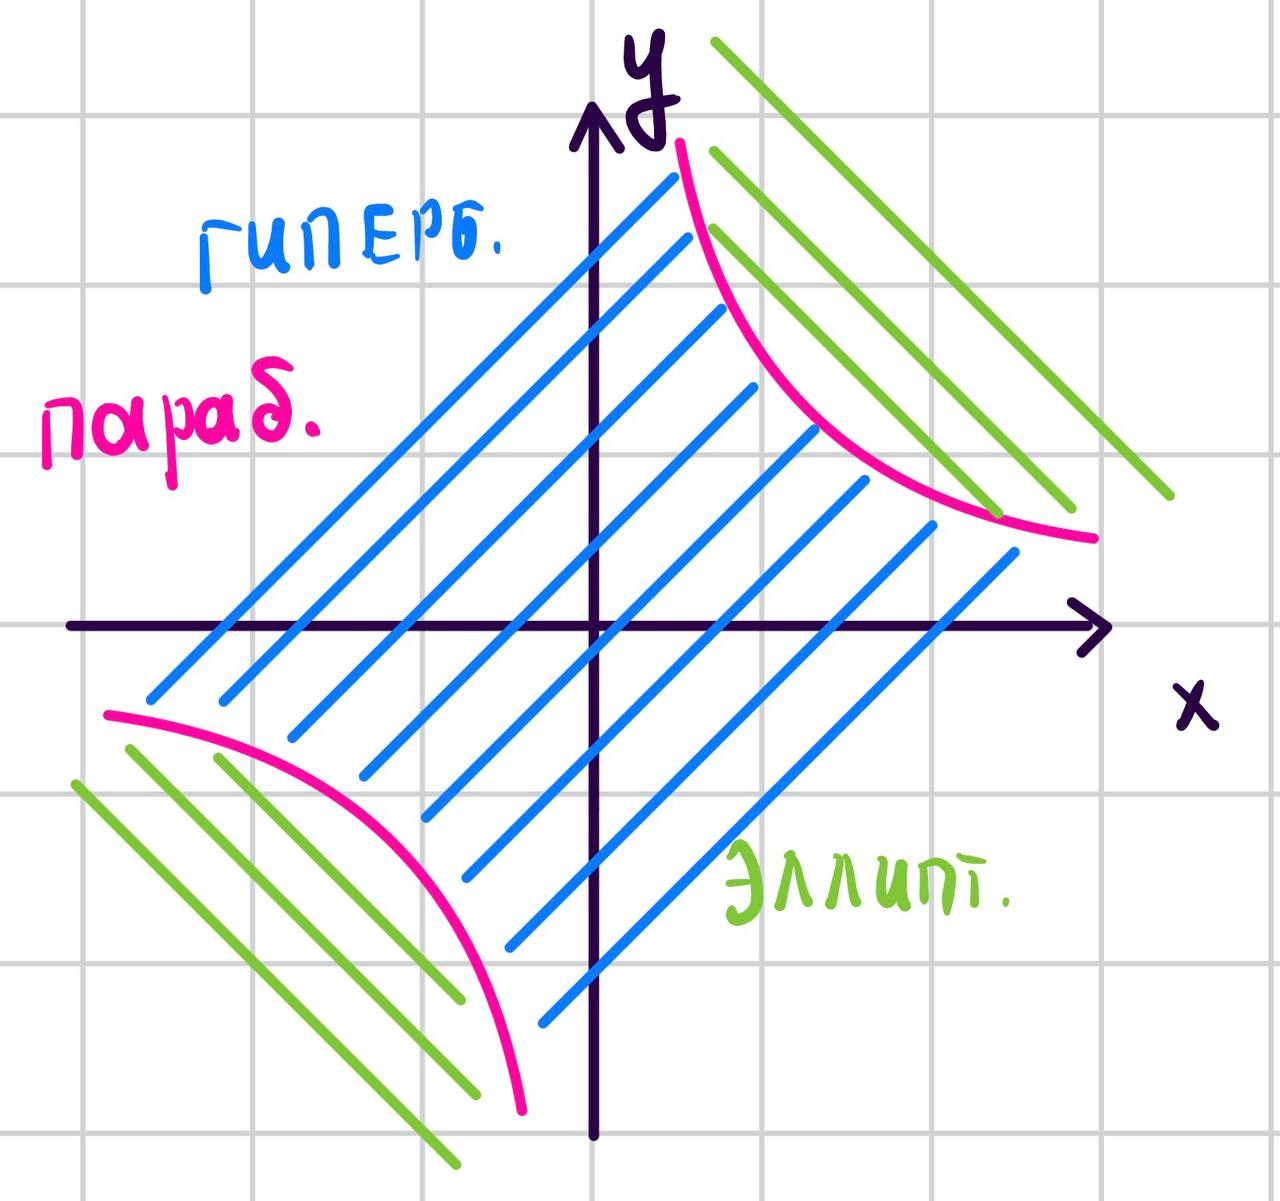
\includegraphics[width=1\linewidth]{pictures/u1.jpg} 
\end{minipage}
\hfill
\begin{minipage}{0.6\textwidth}\raggedleft
\begin{align*}
&\begin{pmatrix}
  y & 1 \\
  1 & x \\
\end{pmatrix} \\
&\Delta_{1} = y, \Delta_{2}=xy-1 \\
&\text{Эллиптический, если} \\ 
& \begin{cases}
 y > 0\\ xy-1>0 \\ 
\end{cases} \text{либо} \begin{cases}
  y < 0\\ xy-1>0
\end{cases}\\
&\text{Гиперболический, если} \\ 
& \begin{cases}
 y < 0 \\ xy-1<0 \\ 
 \end{cases} \text{ либо } \begin{cases}
  y>0 \\ xy-1<0
\end{cases}\\
&\text{Параболлический, если} \\
&xy-1=0 \\ 
\end{align*}
\end{minipage}
\newpage
\item[\text{б})] $(x^{2}+y^{2}-1)u_{xx}+xyu_{yy}-u_{x} = 0.$ \\
  \begin{minipage}{0.3\textwidth}
  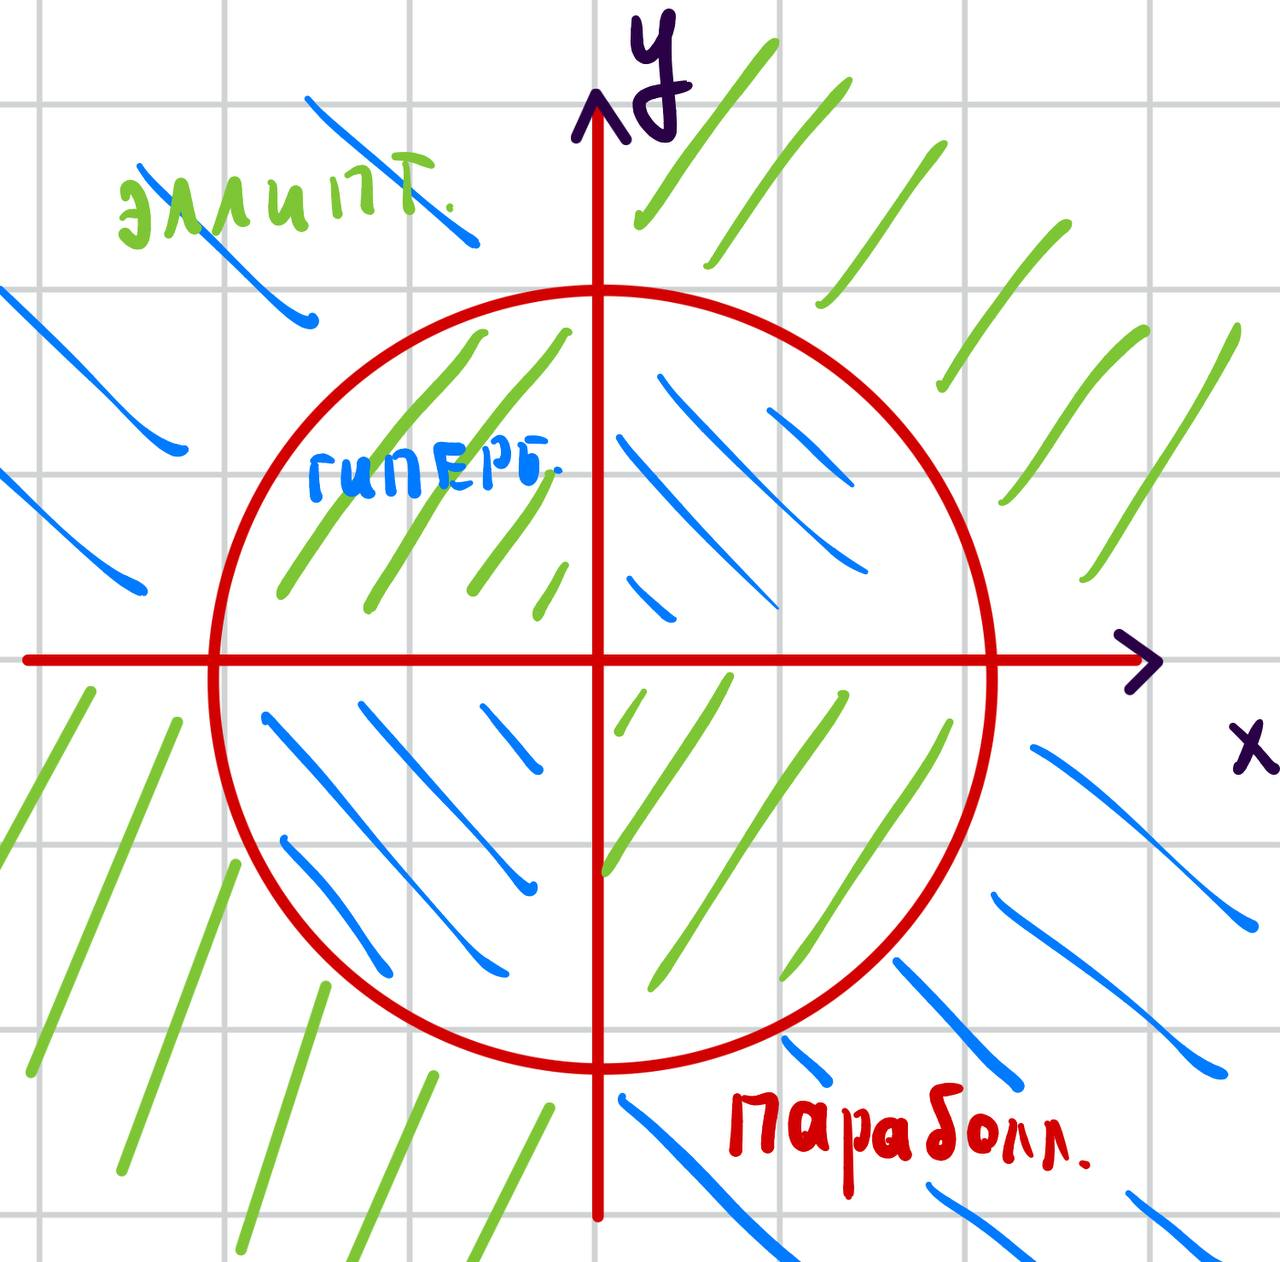
\includegraphics[width=1.3\linewidth]{pictures/u2.jpg} 
  \end{minipage}
  \begin{minipage}{0.6\textwidth}\raggedleft
\begin{align*}
&\begin{pmatrix}
x^{2}+y^{2}-1 & 0 \\
0 & xy \\
\end{pmatrix} \\
&\text{Эллиптический, если} \\ 
&xy(x^{2}+y^{2}-1) > 0\\
&\text{Гиперболический, если} \\ 
&xy(x^{2}+y^{2}-1) < 0\\
&\text{Параболлический, если} \\ 
&xy(x^{2}+y^{2}-1) = 0\\
\end{align*}
  \end{minipage}
\end{enumerate}
\subsection{2} 
$u_{xx}+2\alpha u_{xz}+u_{yy}+4\beta u_{yz}+4u_{zz}=0.$ \\
  \begin{minipage}{0.3\textwidth}
  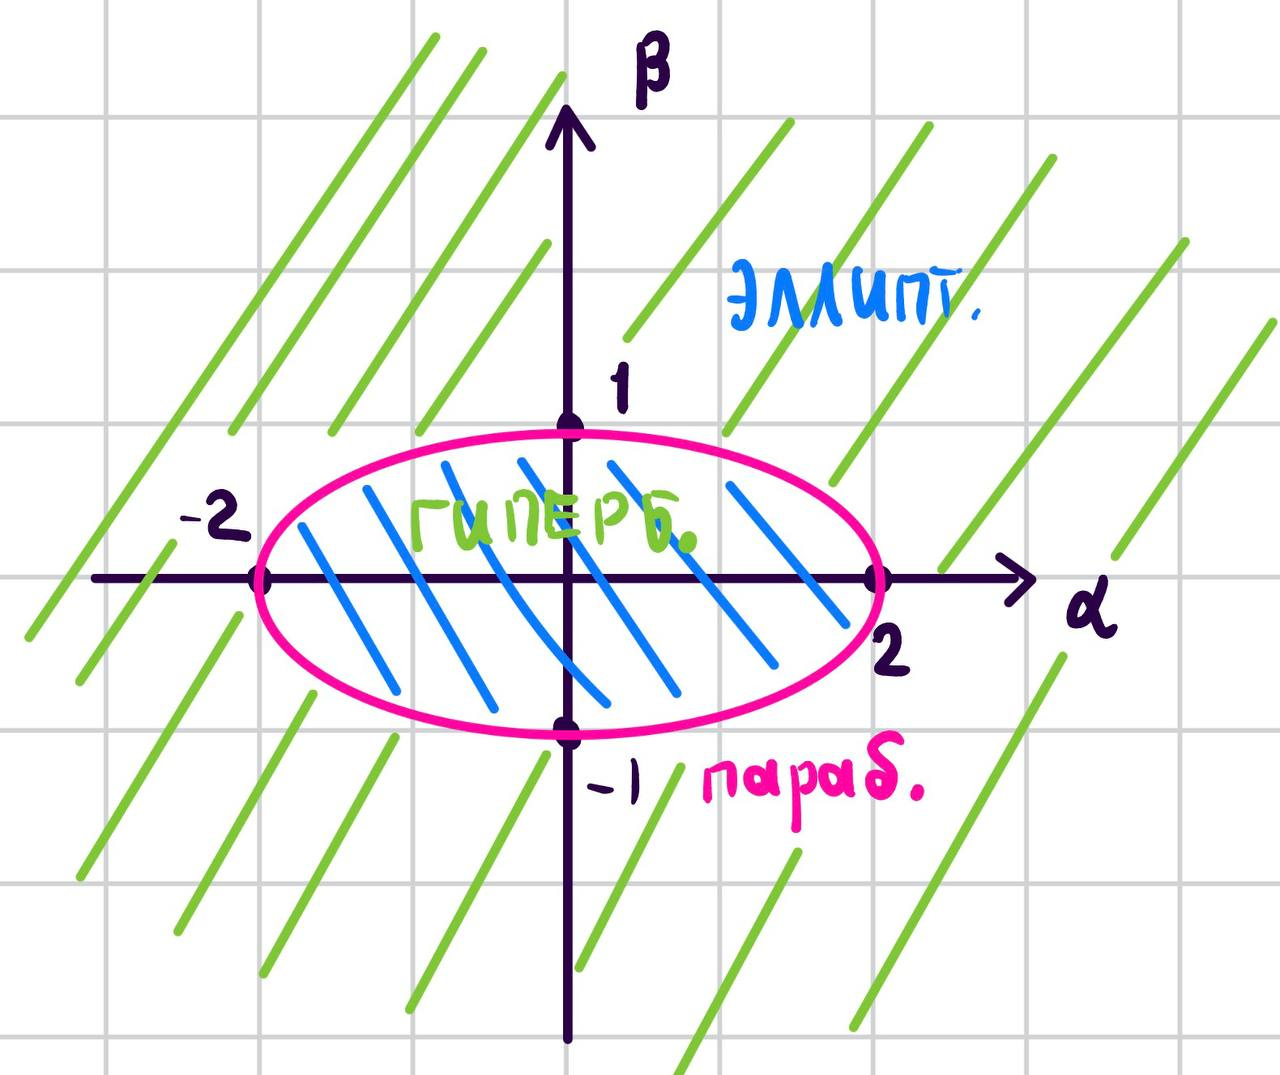
\includegraphics[width=1.4\linewidth]{pictures/u3.jpg} 
  \end{minipage}
  \begin{minipage}{0.6\textwidth}\raggedleft
\begin{align*}
&\begin{pmatrix}
  1 & 0&\alpha \\
  0&1&2\beta \\ 
  \alpha&2\beta&4 \\
\end{pmatrix} \\
&\Delta_{3}=4-4\beta^{2}-\alpha^{2}\\
&\text{Эллиптический, если} \\ 
&4-4\beta^{2}-\alpha^{2}>0\\
&\text{Гиперболический, если} \\ 
&4-4\beta^{2}-\alpha^{2}<0\\
&\text{Параболлический, если} \\ 
&4-4\beta^{2}-\alpha^{2}=0\\
\end{align*}
  \end{minipage}
\subsection{2.1(2)}
$4u_{xx}-4u_{xy}-2u_{yz}+u_{y}+u_{z}=0$
\begin{align*}
&  \left(4 \frac{\partial^{2}}{\partial x^{2}}-4 \frac{\partial^{2}}{\partial x\partial y}-2
  \frac{\partial^{2}}{\partial y\partial z} \right)u+u_{y}+u_{z}=0 \\
 & \left( \left(\underbrace{2\frac{\partial}{\partial x}
    -\frac{\partial}{\partial y}}_{ \frac{\partial}{\partial\xi}}\right)^{2}-\left( 
    \underbrace{\frac{\partial}{\partial y}
 +\frac{\partial}{\partial z}}_{ \frac{\partial}{\partial \mu}}\right)^{2}+\left( \underbrace{
\frac{\partial}{\partial z}}_{ \frac{\partial}{\partial \nu}}\right)^{2}\right)u
  +u_{y}+u_{z}=0\\
 & u_{\xi\xi}-u_{\mu \mu}+u_{\nu \nu}+u_{\mu}=0 \quad \text{гиперболический} \\
 & u = u(x(\xi,\mu\nu),y(\xi,\mu,\nu),z(\xi,\mu,\nu)) \\
 & \frac{\partial u}{\partial \xi} = \frac{\partial u}{\partial x}\underbrace{\frac{\partial x}{\partial \xi}}_{2}+
 \frac{\partial u}{\partial y}\underbrace{\frac{\partial y}{\partial \xi}}_{-1}+
 \frac{\partial u}{\partial z}\underbrace{\frac{\partial z}{\partial \xi}}_{0} \\
 & \frac{\partial u}{\partial \mu} = \frac{\partial u}{\partial x}\underbrace{\frac{\partial x}{\partial \mu}}_{0}+
 \frac{\partial u}{\partial y}\underbrace{\frac{\partial y}{\partial \mu}}_{1}+
 \frac{\partial u}{\partial z}\underbrace{\frac{\partial z}{\partial \mu}}_{1} \\
 & \frac{\partial u}{\partial \nu} = \frac{\partial u}{\partial x}\underbrace{\frac{\partial x}{\partial \nu}}_{0}+
 \frac{\partial u}{\partial y}\underbrace{\frac{\partial y}{\partial \nu}}_{0}+
 \frac{\partial u}{\partial z}\underbrace{\frac{\partial z}{\partial \nu}}_{1} \\
 & \text{Замена} \\
 & \begin{cases}
   x = 2\xi \\ y =-\xi + \mu \\ z = \mu + \nu \\ 
  \end{cases} \\
\end{align*}



\section{Приведение к каноническому виду уравнений 1-го порядка в случае двух независимых переменных
в области}
\subsection{2.11(6)}
$u_{xy}+2xyu_{y}-2xu=0$ \\
\begin{gather*}
 u_{y}=v \\
 v_{x}+2xyv-2xu=0 \quad \text{Продиффиринцируем по $y$} \\
 \frac{\partial}{\partial y}( v_{x}+2xyv-2xu)=0  \ \Rightarrow \ v_{xy}+2xyv_{y}=0 \\
 v_{y}=\tau \\
 \tau_{x}+2xy\tau=0 \quad \frac{d\tau}{dx}=-2xy\tau \Rightarrow \frac{d\tau}{\tau} = -2xydx \\
 \tau = \exp(-x^{2}y)C(y) \qquad v = \int_{0}^{y} C(t)e^{-x^{2}t} \,dt+f(x) \\
 u = \frac{1}{2x}(v_{x}+2xyv) \\
 \boxed{u = \frac{1}{2x}\left(\int_{0}^{y} C(t)(-2xt)e^{-x^{2}t} \,dt+f'(x)+2xy\int_{0}^{y} C(t)e^{-x^{2}t} \,dt+f(x) \right)}\\
\end{gather*}
\subsection{1}
\begin{enumerate}
  \item[\text{а})] $y^{3}u_{xy}-yu_{yy}-3y^{5}u_{x}+(2+3y^{3})u_{y}=0, \ y>0,\ x \in \mathbb{R}^{1};$\\
$u|_{y=1}=1+3x, \quad u_{y}|_{y=1}=3(4+3x),\ x \in \mathbb{R}^{1}.$
\begin{gather*}
  \text{Ур-е характеристик} \\
  -y^{3}dxdy-y(dx)^{2}=0 \quad dx(y^{3}dy+ydx)=0 \\
  \begin{cases}
   dx = 0 \\ y^{3}dy+ydx=0 \\ 
  \end{cases} \Leftrightarrow 
  \begin{cases}
   x = C_{1} \\ y(y'y^{2}+1)=0 \\ 
  \end{cases}\Leftrightarrow 
  \begin{cases}
   C_{1} = x \\ C_{2}=x+ \frac{y^{3}}{3} \\ 
  \end{cases} \\
  \text{Делаем замену} \\
  \begin{cases}
    \xi = x \\ \mu = x + \frac{y^{3}}{3}\\
  \end{cases} \\
  u_{x}=u_{\xi}+u_{\mu} \\ u_{y}=y^{2}u_{\mu} \\
  u_{yy}=y^{4}u_{\mu \mu}+2yu_{\mu} \quad u_{xy}=u_{\xi \mu}y^{2}+u_{\mu \mu}y^{2} \\
  \text{Подставим} \\
  y^{3}(u_{\xi \mu}y^{2}+u_{\mu \mu}y^{2})-y(y^{4}u_{\mu \mu}+2yu_{\mu})-3y^{5}(u_{\xi}+u_{\mu})+
  (2+3y^{3})y^{2}u_{\mu} = 0\\
  y^{5}u_{\xi \mu}-3y^{5}u_{\xi}=0 \quad u_{\xi \mu}-3u_{\xi}=0\\
  u_{\xi}=v \\
  v_{\mu}-3v=0 \quad \frac{dv}{d\mu}=3v \quad v = e^{3\mu}C(\xi) \\
  u_{\xi}=e^{3\mu}C(\xi) \quad du =e^{3\mu}C(\xi)d\xi \\ 
  u=\int_{}^{} C(\xi)e^{3\mu} \,d\xi+f(\mu)=e^{3\mu}g(\xi)+f(\mu) \\
\end{gather*}
  \begin{gather*}
  u=e^{3x+y^{3}}g(x)+f(x+ \frac{y^{3}}{3}) \\
  u|_{y=1} = e^{3x+1}g(x)+f(x+ \frac{1}{3})=1+3x\\
  u_{y}=3y^{2}e^{3x+y^{3}}g(x)+y^{2}f'(x+ \frac{y^{3}}{3}) \\
  u_{y}|_{y=1}=3e^{3x+1}g(x)+f'(x+ \frac{1}{3}) = 3(4+3x)\\
  3+9x-3f(x + \frac{1}{3}) = 3(4+3x)-f'(x+ \frac{1}{3}), \ p = x + \frac{1}{3} \\
  f '(p)=3f(p)+9 \qquad f(p)=e^{3p}C-3 \qquad g(x) = \frac{4+3x-Ce^{3p}}{e^{3x+1}} \\
  g(x) = (4+3x)e^{-3x-1}-C \\
  u=e^{3x+y^{3}}((4+3x)e^{-3x-1}-C)+Ce^{3x+y^{3}}-3=3x+1 \\
  \boxed{u=e^{y^{3}-1}(4+3x)-3}
  \end{gather*}
\item[\text{б})] $x^{2}u_{xx}-9y^{2}u_{yy}+3xu_{x}-3yu_{y}=0, \quad x>1, \ y>1$ \\
  $u|_{x=y}=y^{2 / 3},u_{x}|_{x=y}=y^{-3}+y^{-1 /3}, y>1$ \\
  \begin{gather*}
    \text{Ур-е характеристик} \\
    x^{2}(dy)^{2}-9y^{2}(dx)^{2}=0 \\
    (\frac{dy}{dx})^{2}=( \frac{3y}{x})^{2} \\
    \begin{cases}
     \frac{dy}{y}= \frac{3dx}{x} \\ \frac{dy}{y}= -\frac{3dx}{x} \\
    \end{cases} \Leftrightarrow 
    \begin{cases}
     C_{1} = \frac{y}{x^{3}} \\ C_{2}= yx^{3} \\ 
    \end{cases} \Leftrightarrow 
    \begin{cases}
    \xi = \frac{y}{x^{3}} \\ \mu= yx^{3} \\ 
    \end{cases} \\
    u_{x} = -3u_{\xi} \frac{y}{x^{4}} + 3u_{\mu}yx^{2}, \ u_{y}= \frac{u_{\xi}}{x^{3}} + u_{\mu}x^{3} \\
    u_{xx}=9u_{\xi\xi}y^{2}x^{-8}+9u_{\mu \mu}y^{2}x^{4}-18u_{\xi \mu}x^{-2}y^{2}+12u_{\xi}yx^{-5}+
    6u_{\mu}yx \\
    u_{yy}=u_{\xi\xi}x^{-6}+u_{\mu\mu}x^{6}+2u_{\xi\mu} \\
  \end{gather*}
  \begin{gather*}
    -36u_{\xi\mu}y^{2}+u_{\xi}(12yx^{-3}-9x^{-3}y-3x^{-3}y)+u_{\mu}(6yx^{3}+9yx^{3}-3x^{3}y)=0 \\
    -36u_{\xi\mu}y^{2}+12u_{\mu}yx^{3}=0 \\
    u_{\mu} = v \\
    3v_{\xi}y=vx^{3} \quad 3\frac{dv}{d\xi}= \xi^{-1}v \quad \frac{dv}{v} = \frac{d\xi}{3\xi}\\
    v = \xi^{ \frac{1}{3}}C(\mu) \\
    u = \xi^{ \frac{1}{3}}f(\mu)+g(\xi) \quad 
    u = (x^{-3}y)^{ \frac{1}{3}}f(yx^{3})+g(yx^{-3})\\
    u_{x} = - y^{1 / 3}x^{-2}f(yx^{3})+3xy^{4 /3}f'-3x^{-4}yg' \\
    u|_{x=y}=y^{- \frac{2}{3}}f(y^{4})+g(y^{-2}) = y^{2 / 3}\\ 
    u_{x}|_{x=y}=-y^{-5 /3}f(y^{4})+3y^{7 /3}f'(y^{4})-3y^{-3}g'(y^{-2})=y^{-3}+y^{-1 /3} \\
    \frac{2}{3}y^{-1 /3}= - \frac{2}{3}y^{-5 /3}f(y^{4})+4y^{7 /3}f'(y^{4})-2y^{-3}g'(y^{-2}) \\
    -6y^{7 /3}f'(y^{4})+3y^{7 /3}f'(y^{4})=y^{-3} \quad -3y^{7 /3}f'(y^{4})=y^{-3} \\
    3\frac{df(\mu)}{dy}=- y^{-16/3} \ 3f'(\mu)=-\mu^{-4 /3} \\
    f(y^{4}) = (y^{4})^{-1 /3} + C\\
    y^{-2 /3}(y^{-4 /3}+C)+g(y^{-2})=y^{2 /3} \quad g(y^{-2}) = y^{2 /3} -Cy^{-2 /3}-y^{-2} \\
    f(\mu) = \mu^{-1 /3}+C \quad g(\xi)=\xi^{-1 /3} -C\xi^{1 /3}-\xi \\
    u = \xi^{1 /3}(\mu^{-1 /3}+C)+\xi^{-1 /3} -C\xi^{1 /3}-\xi \\
    u = \xi^{1 /3}\mu^{-1 /3}+\xi^{-1 /3}-\xi \\
    \boxed{u = x^{-2}+y^{-1 /3}x-yx^{-3}}
  \end{gather*} \newpage
\item[\text{в})] $x^{2}u_{xx}-xyu_{xy}-2y^{2}u_{yy}+xu_{x}-2yu_{y}=9xy^{2},\ x>0,\ y>0$ \\
  $u|_{x=1}=3e^{y}, \quad u_{x}|_{x=1}=-y^{2}$ \\
  \begin{gather*}
    \text{Ур-е хар-тик} \\
    x^{2}(dy)^{2}+xydxdy-2y^{2}(dx)^{2} = 0 \\
    ( \frac{dy}{dx})^{2}+ \frac{y}{x} \frac{dy}{dx} -2 (\frac{y}{x})^{2}=0 \\
    \begin{cases}
     \frac{dy}{dx}= -\frac{2y}{x} \\ \frac{dy}{dx} =  \frac{y}{x} 
    \end{cases} \Leftrightarrow
    \begin{cases}
      C_{1} = yx^{2} \\ C_{2} = \frac{y}{x}
    \end{cases} \Leftrightarrow
    \begin{cases}
      \xi = yx^{2} \\ \mu = \frac{y}{x} 
    \end{cases} \\
    u_{x} = 2u_{\xi}yx - u_{\mu}yx^{-2} \qquad u_{y} = u_{\xi}x^{2}+u_{\mu}x^{-1} \\
    u_{xx} = 4u_{\xi\xi}y^{2}x^{2}+u_{\mu\mu}yx^{-4}-4u_{\xi\mu}y^{2}x^{-1}+2u_{\xi}y+2u_{\mu}
    yx^{-3} \\
    u_{yy}= u_{\xi\xi}x^{4}+u_{\mu\mu}x^{-2}+2u_{\xi\mu}x \\
    u_{xy}=2u_{\xi\xi}yx^{3}-u_{\mu\mu}yx^{-3}+u_{\xi\mu}y+2u_{\xi}x-u_{\mu}x^{-2} \\
    \text{После подстановки} \\
    u_{\xi\mu} = -1 \qquad u_{\xi} = v \qquad v_{\mu} = -1 \\
    v = -\mu + C(\xi) \qquad u = -\mu\xi + F(\xi)+G(\mu) \\
    u = -y^{2}x +F(yx^{2})+G(yx^{-1}) \qquad  u_{x}=-y^{2}+2yxF'(yx^{2}) -yx^{-2}G'(yx^{-1}) \\
    u|_{x=1}=-y^{2}+F(y)+G(y) = 3e^{y} \qquad u_{x}|_{x=1}=-y^{2}+2yF'(y)-yG'(y) = -y^{2} \\
   \begin{cases}
    -y^{2}+F(y)+G(y) = 3e^{y} \\ 2F'(y)=G'(y) \\
   \end{cases} \Rightarrow
   \begin{cases}
   -2y + F'(y)+G'(y)=3e^{y} \\ 2F'(y)=G'(y) \\
   \end{cases} \Rightarrow \\
   -2y +3F'(y)=3e^{y} \ \Rightarrow \ F(y)  = e^{y} + \frac{y^{2}}{3}+C \\
   G(y)=3e^{y}+y^{2}-e^{y}- \frac{y^{2}}{3}-C = 2e^{y} + \frac{2y^{2}}{3}-C\\
   \boxed{u = -xy^{2}+e^{yx^{2}}+ \frac{y^{2}x^{4}}{3}+2e^{yx^{-1}}+ \frac{2y^{2}}{3x^{2}}}
  \end{gather*} \newpage
\item[\text{г})] $yu_{xx}+(x-y)u_{xy}-xu_{yy}-u_{x}+u_{y}=0$ \\
  $u|_{y=0}=2x^{2}, \quad u_{y}|_{y=0}=2x, \quad 1<x<4$ \\
  \begin{gather*}
    \text{Ур-е хар-тик} \\
    y(dy)^{2}-(x-y)dxdy-x(dx)^{2}=0 \\
    \begin{cases}
     \frac{dy}{dx}= \frac{x}{y} \\ \frac{dy}{dx} =-1 \\ 
    \end{cases} \Leftrightarrow 
    \begin{cases}
      y^{2}= x^{2} +C_{1} \\ y = -x +C_{2}
    \end{cases} \Leftrightarrow 
    \begin{cases}
      \xi = y^{2}- x^{2} \\ \mu = y+x
    \end{cases} \\
    u_{x}= -2xu_{\xi}+u_{\mu} \qquad u_{y}= 2yu_{\xi}+u_{\mu} \\
    u_{xx}=4x^{2}u_{\xi\xi}+u_{\mu\mu}-4xu_{\xi\mu}-2u_{\xi} \\
    u_{yy}=4y^{2}u_{\xi\xi}+u_{\mu\mu}+4yu_{\xi\mu}+2u_{\xi} \\
    u_{xy}=-4yxu_{\xi\xi}+u_{\mu\mu}+2(y-x)u_{\xi\mu} \\
    \text{После подстановки} \\
    2u_{\xi\mu}\mu^{2}=0 \quad u_{\xi}=v \quad  v_{\mu} = 0 \\
    v = C(\xi) \qquad u = f(\xi)+g(\mu) \qquad u = f(y^{2}-x^{2})+g(y+x) \\
    u_{y} = 2yf'(y^{2}-x^{2})+g'(y+x) \\
    u|_{y=0} = f(-x^{2}) + g(x)=2x^{2} \qquad u_{y}|_{y=0}=  g'(x) =2x \\
    g(x)=x^{2}+C \qquad f(-x^{2})+x^{2}+C=2x^{2} \ \Rightarrow \ f(-x^{2}) = x^{2}-C \\
    u=(y+x)^{2}+x^{2}-y^{2} \\
    \boxed{u=2x^{2}+2xy} \\
  \end{gather*} \newpage
\item[\text{д})] $y^{4}u_{yy}+y^{2}u_{xy}-2u_{xx}+2y^{3}u_{y}=0$ \\
  $u|_{y=1}=x^{2}+5, \quad u_{y}|_{y=1}=2x-6, \ 1<x<2$ \\
  \begin{gather*}
    \text{Ур-е хар-тик} \\
    y^{4}(dx)^{2}-y^{2}dxdy-2(dy)^{2}=0 \\
    \begin{cases}
      y' = -y^{2} \\ y' =\frac{1}{2}y^{2} 
    \end{cases} \Leftrightarrow
    \begin{cases}
      C_{1} = x - \frac{1}{y} \\ C_{2} = x + \frac{2}{y} \\
    \end{cases} \Rightarrow
    \begin{cases}
      \xi = x - \frac{1}{y} \\ \mu = x + \frac{2}{y} \\
    \end{cases} \\
  u_{x} = u_{\xi} +u_{\mu} \qquad u_{y} = \frac{u_{\xi}}{y^{2}} - \frac{2u_{\mu}}{y^{2}} \\
  u_{xx}=u_{\xi\xi}+2u_{\xi\mu}+u_{\mu\mu} \qquad u_{yy}= \frac{u_{\xi\xi}}{y^{4}}+ \frac{4u_{\mu\mu}}{y^{4}}
  - \frac{4u_{\xi\mu}}{y^{4}}-2 \frac{u_{\xi}}{y^{3}}+ 4 \frac{u_{\mu}}{y^{3}} \\
  u_{xy}= \frac{u_{\xi\xi}}{y^{2}} - 2 \frac{u_{\mu\mu}}{y^{2}} - \frac{u_{\xi\mu}}{y^{2}} \\
  u_{\xi\mu} = 0 \\
  u = f(\xi)+g(\mu) \quad u = f(x - \frac{1}{y})+g(x+ \frac{2}{y}) \\
  u_{y}=y^{-2}f'(x- \frac{1}{y})-2y^{-2}g'(x+ \frac{2}{y}) \\
  u|_{y=1}=f(x-1)+g(x+2)=x^{2}+5 \\ u_{y}|_{y=1}=f'(x-1)-2g'(x+2)=2x-6 \\
  \begin{cases}
    f(x-1)+g(x+2)=x^{2}+5 \\ f'(x-1)-2g'(x+2)=2x-6
  \end{cases} \Rightarrow \begin{cases}
    f(x-1) = x^{2}+5-g(x+2) \\ 2x-g'(x+2)-2g'(x)=2x-6
  \end{cases} \Rightarrow \\ \Rightarrow \begin{cases}
  f(x-1) = x^{2}+5-g(x+2) \\ g'(x+2) = 2
  \end{cases} \Rightarrow \begin{cases}
    f(x-1) = x^{2} -2x + 1 - C \\ g(x+2) = 2x+4+C
  \end{cases} \Rightarrow \\ \Rightarrow \begin{cases}
    f(x-1)=(x-1)^{2}-C \\ g(x+2) = 2(x+2) +C
  \end{cases} \Rightarrow \begin{cases}
    f(a)=a^{2}-C \\ g(b) = 2b+C
  \end{cases} \\
  \boxed{u=(x- \frac{1}{y})^{2}+2(x+ \frac{2}{y})}
\end{gather*}
\end{enumerate}

\subsection{2}
$x^{2}u_{xx}-4y^{2}u_{yy}+xu_{x}-4yu_{y}=0, \quad \frac{1}{x^{2}}<y<x^{2}, \ x>0$ 

$u|_{y= \frac{1}{x^{2}}}= 1 +2x^{4}, \ u|_{y=x^{2}} = 2 + x^{4}$ 

\begin{gather*}
  \text{Ур-е характеристик} \\
  x^{2}(dy)^{2}-4y^{2}(dx)^{2} \\
  \begin{cases}
    \frac{dx}{x} = \frac{dy}{2y} \\ \frac{dx}{x}= - \frac{dy}{2y} \\
  \end{cases} \Leftrightarrow
  \begin{cases}
    x = \sqrt{y}C_{1} \\ x = \frac{1}{\sqrt{y}}C_{2} \\
  \end{cases} \\
  \text{Замена} \\
  \begin{cases}
    \mu =\sqrt{y}x \\ \xi =\frac{x}{\sqrt{y}} \\
  \end{cases} \\
  u_{x}=u_{\xi} \frac{1}{\sqrt{y}}+ u_{\mu}\sqrt{y}, \quad u_{y}= - 
  \frac{x}{2 \sqrt{y^{3}}}u_{\xi} + u_{\mu} \frac{x}{2 \sqrt{y}} \\
  u_{xx}= \frac{u_{\xi \xi}}{y} + u_{\mu \mu} y + 2 u_{\xi \mu} \\
  u_{yy}=u_{\xi \xi} \cdot \frac{x^{2}}{4y^{3}} + u_{\mu \mu} \cdot \frac{x^{2}}{4y} - u_{\xi \mu}
  \cdot \frac{x^{2}}{2 y^{2}} - u_{\mu} \frac{x}{4 \sqrt{y^{3}}} + u_{\xi} \frac{3x}{4 \sqrt{y^{5}}} \\
  \text{Подставим} \\
  x^{2}(\frac{u_{\xi \xi}}{y} + u_{\mu \mu} y + 2 u_{\xi \mu})-4y^{2}(u_{\xi \xi} \cdot \frac{1}{4y^{3}} + u_{\mu \mu} \cdot \frac{x^{2}}{4y} - u_{\xi \mu}
  \cdot \frac{x}{2 y^{2}} - u_{\mu} \frac{x}{4 \sqrt{y^{3}}} + u_{\xi} \frac{3}{4 \sqrt{y^{5}}}) +\\
  +x(u_{\xi} \frac{1}{\sqrt{y}}+ u_{\mu}\sqrt{y})-4y(- 
  \frac{1}{2 \sqrt{y^{3}}}u_{\xi} + u_{\mu} \frac{x}{2 \sqrt{y}} ) = 0 \\
  4x^{2}u_{\xi\mu}=0 \ \Rightarrow \ u_{\xi\mu}=0 \\
  u = f(\xi)+g(\mu) \qquad u = f(\frac{x}{\sqrt{y}})+g(\sqrt{y}x) \\
  u|_{y=x^{-2}}=f(x^{2})+g(1)=1+2x^{4} \qquad u|_{y=x^{2}}=f(1)+g(x^{2})=2+x^{4} \\
\end{gather*} \\
\begin{gather*}
  \begin{cases}
  f(x^{2})+g(1)=1+2x^{4} \\ f(1)+g(x^{2})=2+x^{4}
  \end{cases} \Rightarrow \begin{cases}
    f(x^{2})=1+2x^{4}-g(1) \\ g(x^{2})=x^{4}-1+g(1)
  \end{cases} \Rightarrow \\
  \Rightarrow \begin{cases}
    f(a)=2a^{2}+C \\ g(b)=b^{2}-C
  \end{cases} \\
  \boxed{u= 2\frac{x^{2}}{y}+yx^{2}}
\end{gather*}
\subsection{3}
$u_{yy}-u_{xx}=0$ \\
$u|_{y=0}=u_{0}(x),\ u_{y}|_{y=0}=u_{1}(x), \ 0 < x < 1, \ u_{0}(x) \in C^{2}(0;1), u_{1}(x)
 \in C_{1}(0;1)$ \\ 
\begin{gather*}
  \text{максимальная область, где $\exists$! реш} \\ 
  \begin{cases}
   0 < x + y < 1 \\ 0< x-y<1 \\ 
  \end{cases}
\end{gather*}


\newpage

\section{Волновое уравнение}
\subsection{1}
\[
\begin{cases}
 4u_{tt} = u_{xx}+4t^{2} \cos(2x) \\ u|_{t=0} = e^{x}, \ u_{t}|_{t=0} = x^{2} 
\end{cases}
\] \\
\begin{gather*}
  u_{\text{частн}}= f(t) \cos(2x) \\ 
  4f'' \cos(2x) = -4f \cos(2x) +4t^{2} \cos(2x) \\ 
  f''=-f+t^{2} \\
  f = \alpha t^{2} + \beta t + \gamma \quad 2\alpha=-\alpha t^{2} - \beta t - \gamma + t^{2}\\ 
  \alpha = 1, \ \beta = 0, \ \gamma = -2 \\
  u_{\text{частн}} = (t^{2}-2) \cos(2x) \\
  u = (t^{2}-2)\cos(2x) + v(x,t) \\
  \begin{cases}
   4v_{tt}=v_{xx} \\ v|_{t=0}=e^{x}+2\cos(2x) \\ v_{t}|_{t=0} = x^{2} \\
  \end{cases} \\
  \boxed{v(x,t)= \frac{1}{2}(e^{x + \frac{t}{2}}+2\cos(2x+t)+e^{x -\frac{t}{2} }+2\cos(2x-t))
  + \int_{x- \frac{t}{2}}^{x +\frac{t}{2}} \xi^{2} \,d\xi} \\
\end{gather*}

\subsection{2}
$u_{tt}=a^{2}u_{xx}, \quad x \in \mathbb{R}^{1}, \quad t>0$ \\
\begin{enumerate}
  \item[\text{а})] $u|_{t=0}=\varphi(x), \ u_{t}|_{t=0}=0;$ \\
    \begin{gather*}
      \text{Ф-ла Даламбера} \\
      u(x,t) = \frac{\varphi(x+at)-\varphi(x-at)}{2} \\
    \end{gather*}
    \begin{minipage}{0.4\textwidth}
  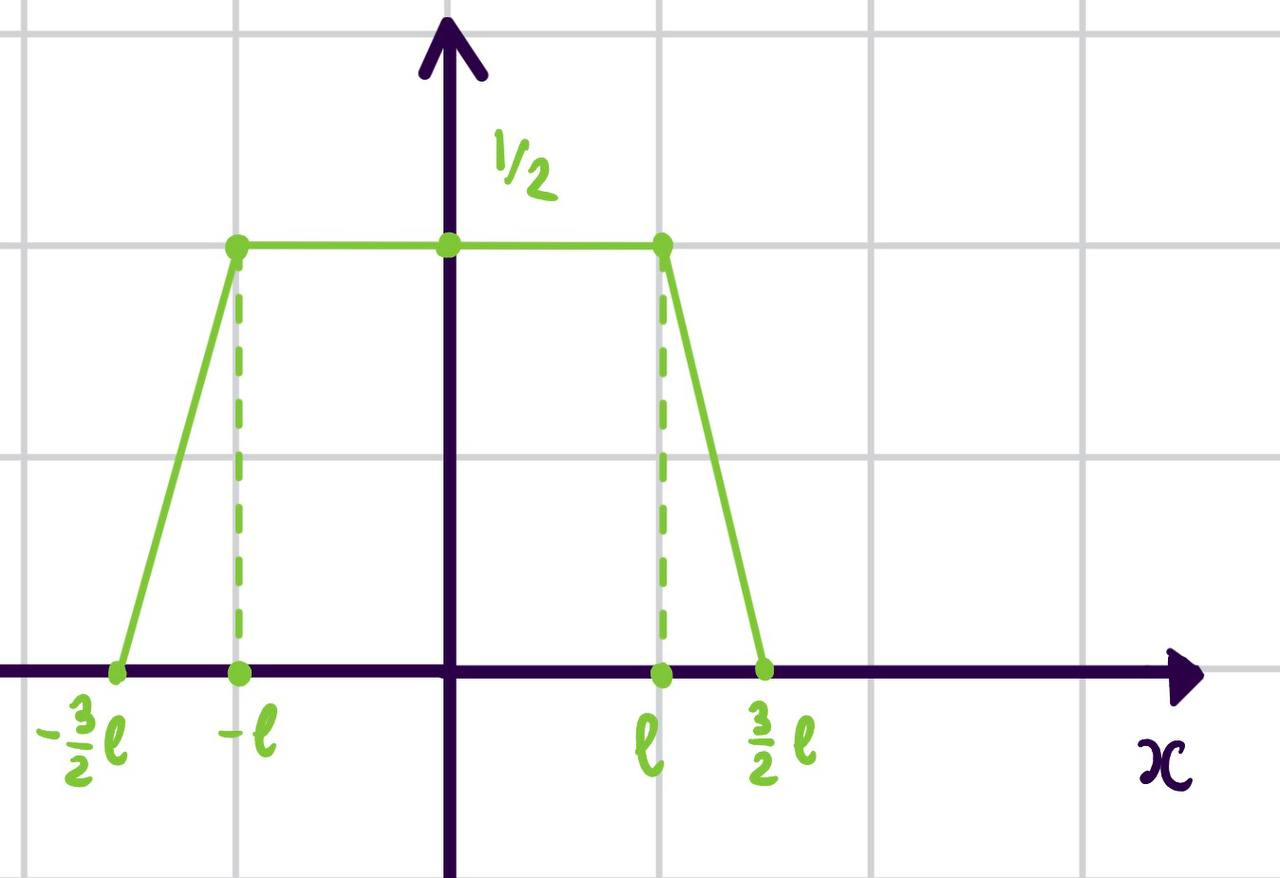
\includegraphics[width=1\linewidth]{pictures/u4.jpg} 
    \end{minipage}
    \begin{minipage}{0.4\textwidth}\raggedleft
      \begin{gather*}
        t = \frac{l}{2a} \\
        u(x,t) = \frac{\varphi(x+ \frac{l}{2})- \varphi(x -\frac{l}{2})}{2} \\
      \end{gather*}
    \end{minipage} \\
    \begin{minipage}{0.4\textwidth}
  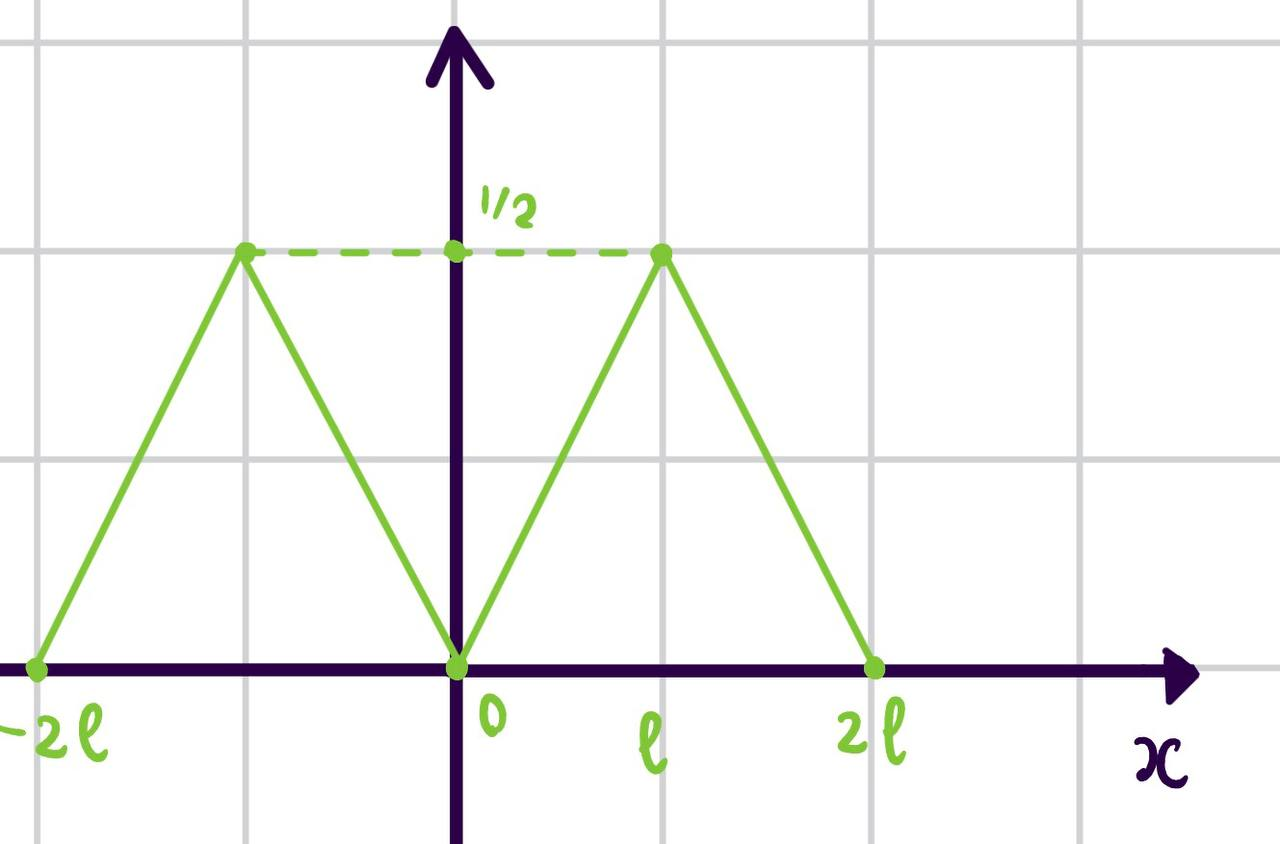
\includegraphics[width=1\linewidth]{pictures/u5.jpg} 
    \end{minipage}
    \begin{minipage}{0.4\textwidth}\raggedleft
      \begin{gather*}
        t = \frac{l}{a} \\
        u(x,t) = \frac{\varphi(x+ l)- \varphi(x -l)}{2} \\
      \end{gather*}
    \end{minipage} \\
    \begin{minipage}{0.4\textwidth}
  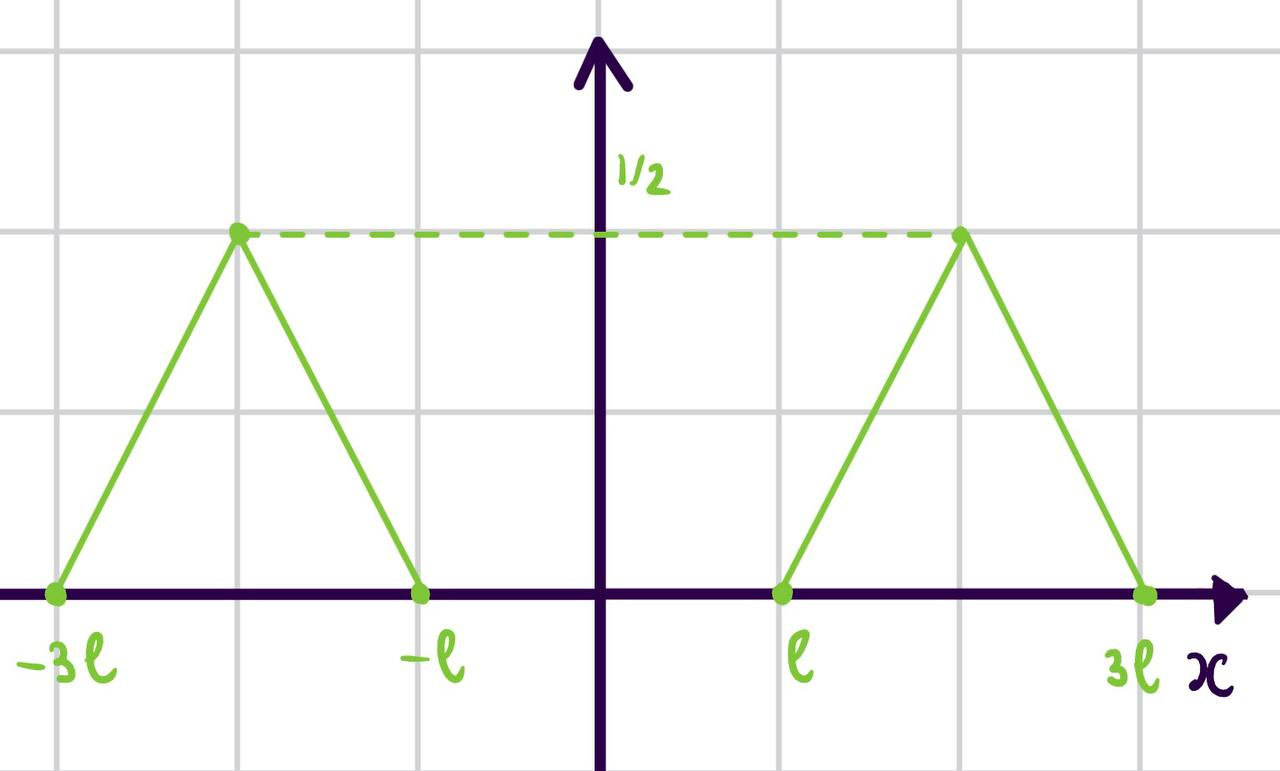
\includegraphics[width=1\linewidth]{pictures/u6.jpg} 
    \end{minipage}
    \begin{minipage}{0.4\textwidth}\raggedleft
      \begin{gather*}
        t = \frac{2l}{a} \\
        u(x,t) = \frac{\varphi(x+ 2l)- \varphi(x -l)}{2} \\
      \end{gather*}
    \end{minipage} \\
  \item[\text{б})] $u|_{t=0}=0, \ u_{t}|_{t=0}= \psi(x)=\theta(l-|x|) \\ 
    l = \text{const} >0 \quad \theta(x) = \begin{cases}
    1, \ x \geq 0 \\ 0, \ x < 0
  \end{cases}$ \\
  \begin{gather*}
    \text{Общее решение} \\
      u(x,t) = \frac{1}{2a}\int_{x-at}^{x+at} \psi(\xi) \,d\xi \\
  \end{gather*}
\end{enumerate}
    \begin{minipage}{0.4\textwidth}
  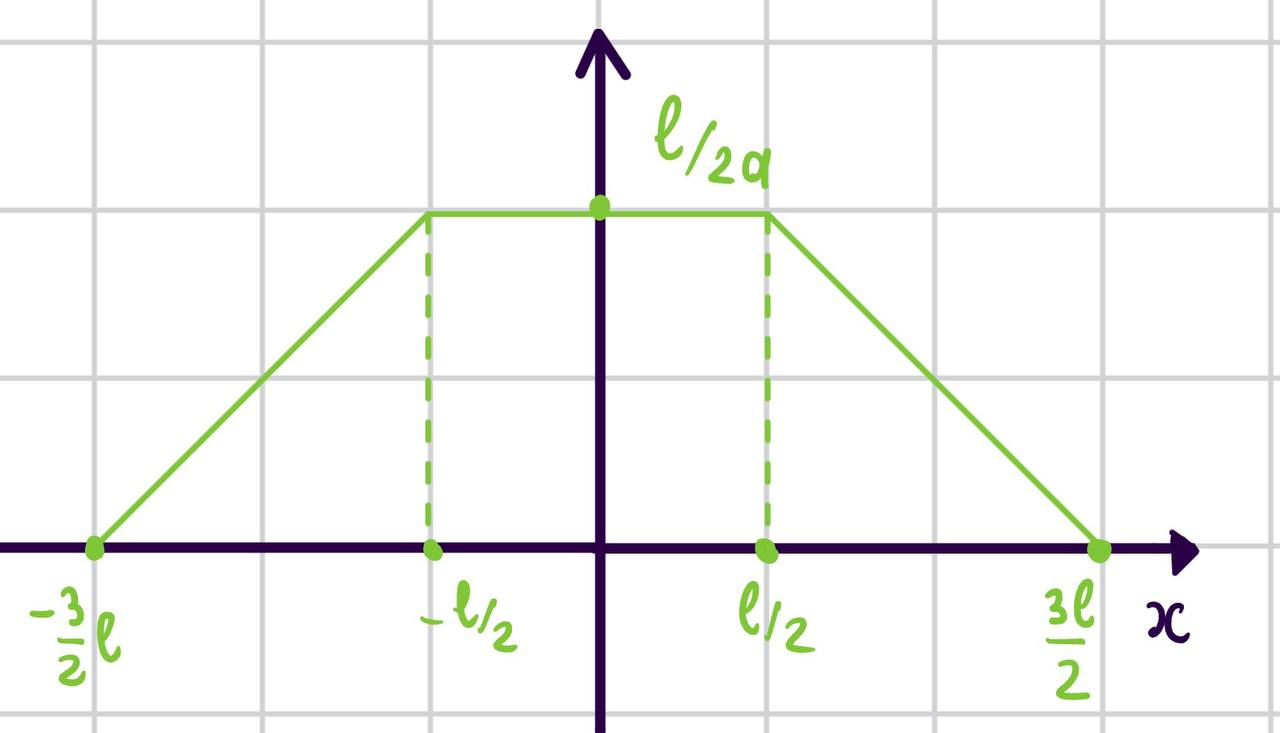
\includegraphics[width=1\linewidth]{pictures/u7.jpg} 
    \end{minipage}
    \begin{minipage}{0.4\textwidth}\raggedleft
      \begin{gather*}
        t = \frac{l}{2a} \\
        \begin{split}
        u(x,t) &= \frac{1}{2a} \int_{x- \frac{l}{2}}^{x + \frac{l}{2}} \theta(l -|\xi| )\,d\xi \\
               &= \frac{1}{2a} \text{length}\left([x-\frac{l}{2},x+\frac{l}{2}]\cup [-l,l]\right)
        \end{split}
      \end{gather*}
    \end{minipage} \\
    \begin{minipage}{0.4\textwidth}
  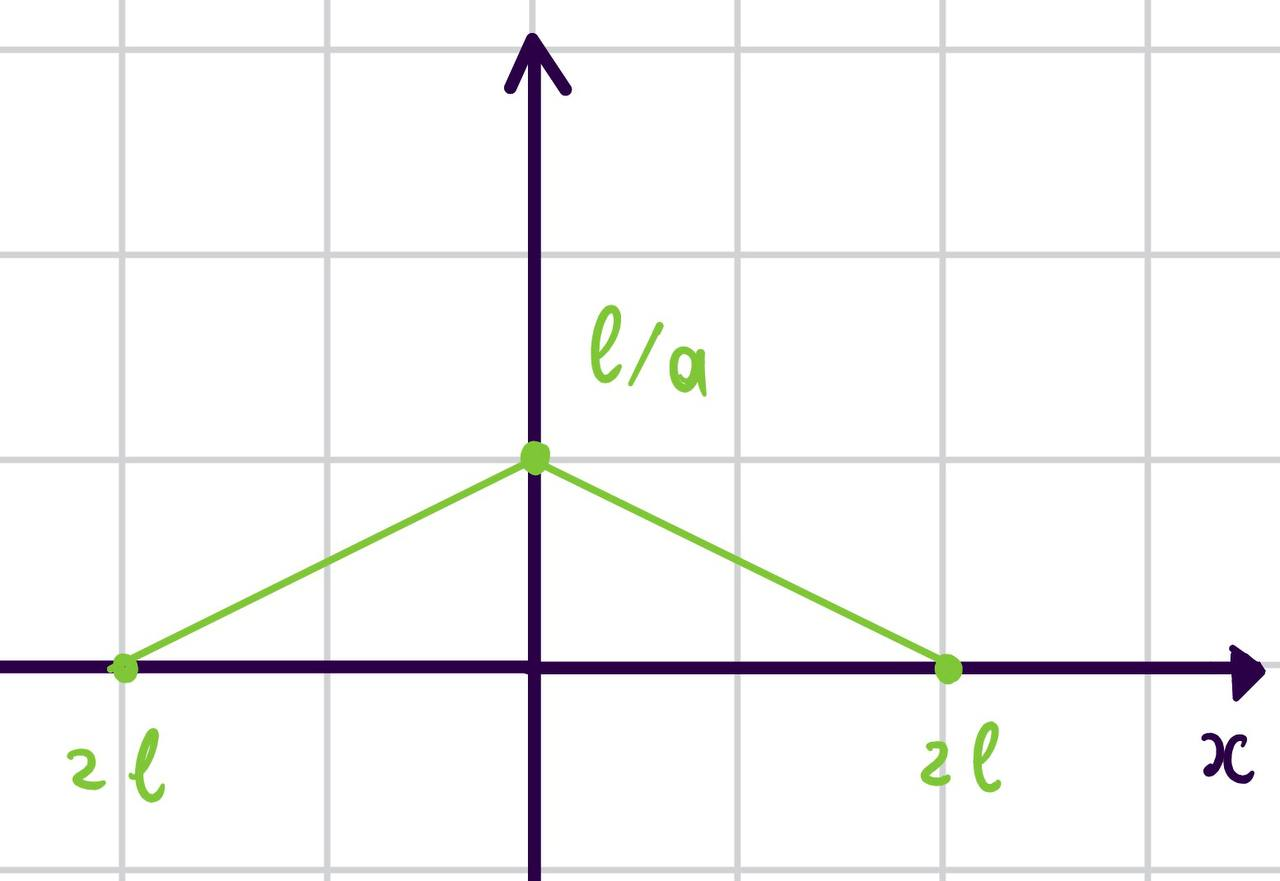
\includegraphics[width=1\linewidth]{pictures/u8.jpg} 
    \end{minipage}
    \begin{minipage}{0.4\textwidth}\raggedleft
      \begin{gather*}
        t = \frac{l}{a} \\
        \begin{split}
        u(x,t) &= \frac{1}{2a} \int_{x- l}^{x + l} \theta(l -|\xi| )\,d\xi \\
               &= \frac{1}{2a} \text{length}\left([x-l,x+l]\cup [-l,l]\right)
        \end{split}
      \end{gather*}
    \end{minipage} \\
    \begin{minipage}{0.4\textwidth}
  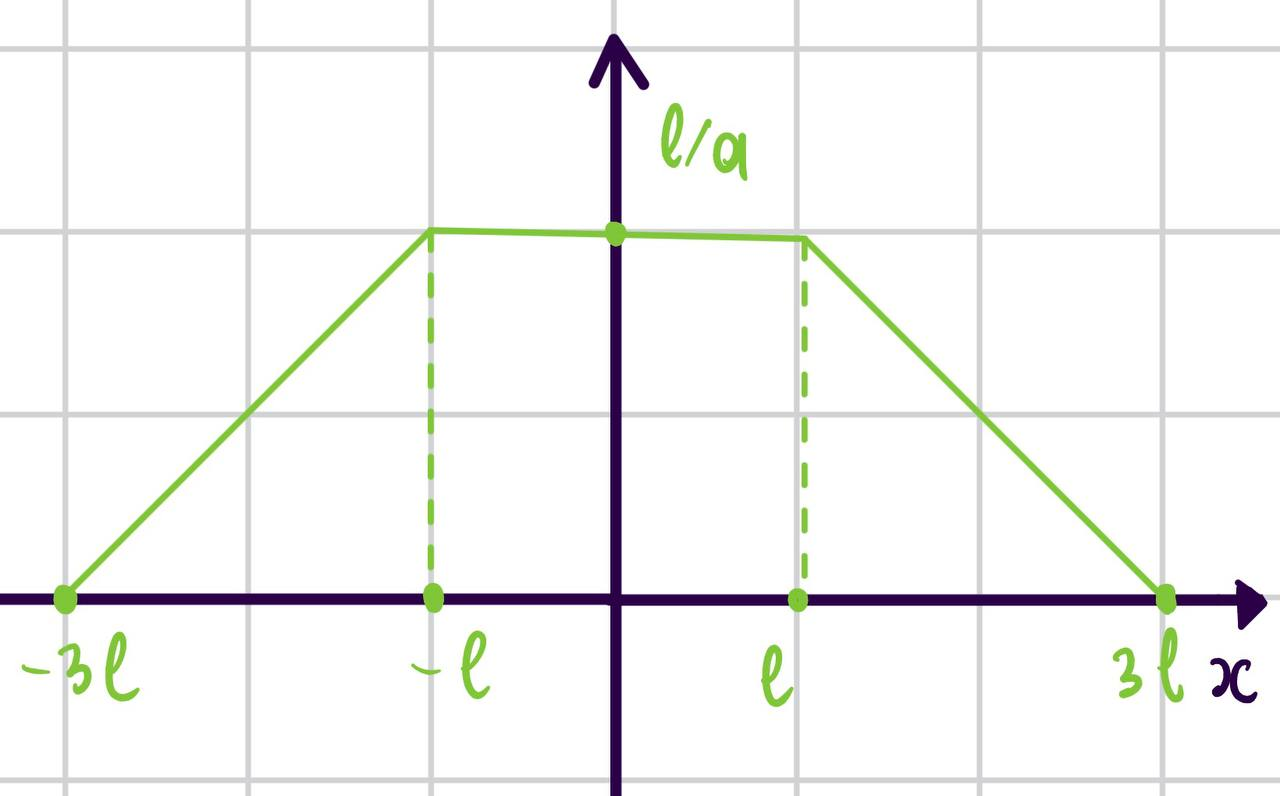
\includegraphics[width=1\linewidth]{pictures/u9.jpg} 
    \end{minipage}
    \begin{minipage}{0.4\textwidth}\raggedleft
      \begin{gather*}
        t = \frac{2l}{a} \\
        \begin{split}
        u(x,t) &= \frac{1}{2a} \int_{x- 2l}^{x + 2l} \theta(l -|\xi| )\,d\xi \\
               &= \frac{1}{2a} \text{length}\left([x-2l,x+2l]\cup [-l,l]\right)
        \end{split}
      \end{gather*}
    \end{minipage} \\
\subsection{3}
\begin{enumerate}
  \item[\text{б})] $u_{tt} = u_{xx} +xe^{t}, \quad x>0,t>0$ \\
$u|_{t=0} = 1=x, \quad u_{t}|_{t=0} = 4-5x, x \geq 0$ \\
$(2u+u_{x})|_{x=0}=(1+t)e^{t}+2+t-3t^{2}, \quad t \geq 0$ \\
\begin{gather*}
  \text{Ищем частные решения} \\
  u_{\text{частн}} = xe^{t} \\
  \text{Сводим ур-е у однородному} \\
  u = xe^{t} + v(x,t) \\
  v_{tt} = v_{xx} \qquad v|_{t=0} = (u - xe^{t})|_{t=0} = 1+x-x=1 \\
  v_{t}|_{t=0}=(u_{t}-xe^{t})|_{t=0}=4-5x-x=4-6x \\
  (2v+v_{x})|_{x=0} = (2u+u_{x}-2xe^{t}-e^{t})|_{x=0} = te^{t}+2+t-3t^{2}, \ t \geq 0 \\
v = f(x+t) + g(x-t) \\
\text{Ищем решение в области $x \geq t$} \\
v|_{t=0} = f(x)+g(x) = 1 \qquad v_{t}|_{t=0} = f'(x) - g'(x) = 4 - 6x, \ x>= 0 \\
f'(x) + g'(x) = 0, \qquad \text{складываем} \\
2f'(x)=4-6x \qquad 2f'(x) = 4-6x \qquad f'(x) = 2-3x \\
\boxed{f(x)=2x -\frac{3x^{2}}{2}+A; \qquad g(x) = 1-2x+ \frac{3x^{2}}{2}-A} \\
v = 2(x+t) - \frac{3}{2}(x+t)^{2}+A+1-2(x-t)+ \frac{3}{2}(x-t)^{2}-A, \ x \geq t \\
\text{Ихем решения при $x < t$} \\
\begin{split}
  (2v+v_{x})|_{x=0} &= 2f(t)+2g(-t)+ f'(t) + g'(-t) = \\
                    &= te^{t} +2+t -3t^{2}, \ t>= 0 \\
\end{split} \\
4t-3t^{2}+2A+2g(-t)+2-3t+g'(-t) = te^{t}+2+t-3t^{2} \\
g'(t)+2g(-t)=te^{t}-2A \qquad -t = p < 0 \\
\end{gather*}
\begin{gather*}
g'(p)+2g(p)=-pe^{t}-2A \\
  g_{\text{частн}_{1}} = (\alpha p + \beta ) e^{-p} \\
  \alpha e^{-p}- (\alpha p +\beta)e^{-p}+2(\alpha p + \beta)e^{-p} = -pe^{-p} \\
  \alpha +2\alpha = -1 \qquad \alpha = -1 \qquad \alpha - \beta +2 \beta = 0 \\
  \beta = -\alpha = 1 \\
  g_{\text{частн}_{1}} = (1-p)e^{-p} \qquad g_{\text{частн}_{2}}=-A \\
  g(p) = ce^{-2p}+(1-p)e^{-p}-A, \quad p < 0 \\
  \text{Сшивка(склейка)} \\
  g(+0)= g(-0) \\
  1-A=C+1-A \Rightarrow C = 0 \\
  \text{Ответ} \\
  \boxed{u(x,t)=xe^{t}+2(x+t)- \frac{3}{2}(x+t)^{2} +
  \begin{cases}
   1-2(x-t) + \frac{3}{2}(x-t)^{2}, \quad x \geq t \\
   (1-(x-t))e^{-(x-t)}, \quad x <t \\
\end{cases}}
\end{gather*}
\item[\text{г})] $u_{tt}+u_{xt}-2u_{xx}=0, \quad x >0, \ t>0$ \\
  $u|_{t=0}=\sh{x}+\arctg{x}, \ u_{t}|_{t=0}= \ch{x}- \frac{2}{1+x^{2}}, \ x \geq 0$ \\
  $u_{x}\_{x=0}=\ch{x}+1, \ t \geq 0$ \\
  \begin{gather*}
    (dx)^{2}-dxdt-2(dt)^{2}=0 \quad (dx-2dt)(dx+dt) = 0 \\
    \begin{cases}
     x = 2t + C_{1} \\ x = -t + C_{2} \\
    \end{cases} \Leftrightarrow
    \begin{cases}
     \xi = x-2t \\ \mu = x=t \\ 
    \end{cases} \\
    u_{x} = u_{\xi} + u_{\mu} \quad u_{t} = -2u_{\xi} + u_{\mu} \\
    u_{xx} = u_{\xi\xi} + u_{\mu\mu} + 2u_{\xi\mu} \\ 
    u_{tt} = 4u_{\xi\xi} + u_{\mu\mu} -4u_{\xi\mu} \\
    u_{xt} = -2u_{\xi\xi}+u_{\mu\mu}-u_{\xi\mu} \\
  \end{gather*}
  \begin{gather*}
    \text{Подставляем} \\
    u_{\xi\mu} = 0 \\
    u = f(\xi)+g(\mu) = f(x-2t) +g(x+t) \\
    u|_{t=0}=f(x)+g(x)= \sh{x} + \arctg{x} \Rightarrow f'(x) + g(x) + \ch{x} = \frac{1}{1+x^{2}} \\
    u'_{t}|_{t=0}=-2f'(x)+g'(x)= \ch{x} - \frac{2}{1+x^{2}} \\
    3f'(x) = \frac{3}{1+x^{2}} \\
    \boxed{f(x) = \arctg{x} +A \qquad g(x) = \sh{x} - A, \ x \geq 0} \\
    u_{x}|_{x=0} = -2tf'(t) + g'(t) = \ch{t} + 1 \\
    f'(-2t) + \ch{t} = \ch{t} +1\\ 
    -2t =z \quad f'(z) = 1 \quad f(z) = z + C, \ z < 0 \\
    f(+0) = f(-0) \Rightarrow C=A \\
    \boxed{u(x,t) = \sh{(x+t)} + 
      \begin{cases}
        \arctg{(x-2t)}, \quad x-2t \geq 0\\ x-2t, \quad x-2t < 0 \\
    \end{cases}}
  \end{gather*}
\end{enumerate}

\end{document}
